\documentclass[11pt, a4paper]{article}
\usepackage[T1]{fontenc}
\usepackage[utf8]{inputenc}
\usepackage{lmodern}
\usepackage[margin=2cm, top=2.5cm, bottom=2.5cm, headheight=14pt]{geometry}
\usepackage{amsmath}
\usepackage{amssymb}
\usepackage[table,dvipsnames]{xcolor}
\usepackage{tikz}
\usetikzlibrary{calc, patterns, shadows}
\usepackage{tcolorbox}
\tcbuselibrary{breakable}
\usepackage{tabularx}
\usepackage{enumitem}
\usepackage{parskip}
\usepackage{titlesec}
\usepackage{fancyhdr}
\usepackage{framed}

\definecolor{accent}{RGB}{29,78,216}
\definecolor{accentlight}{RGB}{239,246,255}
\definecolor{accentmid}{RGB}{96,165,250}
\definecolor{slate}{RGB}{71,85,105}
\definecolor{slatelight}{RGB}{148,163,184}
\definecolor{grass}{RGB}{187,224,163}
\definecolor{earthbrown}{RGB}{161,122,86}
\definecolor{darkearth}{RGB}{120,85,55}
\definecolor{skyblue}{RGB}{186,230,253}
\definecolor{steelgray}{RGB}{148,163,184}
\definecolor{rockgray}{RGB}{203,213,225}
\definecolor{burlywood}{RGB}{222,184,135}

\newcommand{\blank}[1]{\underline{\hspace{#1}}}
\newcommand{\answerline}{\par\vspace{0.5cm}\noindent\rule{\linewidth}{0.4pt}\par\vspace{0.1cm}}

\tcbset{
  problem/.style={colback=accentlight, colframe=accent, leftrule=4pt,
    toprule=0.5pt, bottomrule=0.5pt, rightrule=0.5pt,
    left=8pt, right=8pt, top=6pt, bottom=6pt, breakable},
  answerbox/.style={colback=white, colframe=slatelight,
    left=6pt, right=6pt, top=6pt, bottom=6pt, breakable}
}

\titleformat{\section}{\large\bfseries\color{accent}}{}{0em}{}[\color{accentmid}\titlerule]
\titlespacing{\section}{0pt}{14pt}{6pt}

\pagestyle{fancy}
\fancyhf{}
\fancyhead[L]{\small\color{slate}Math 9 --- Number Unit: Real World Problems}
\fancyhead[R]{\small\color{slate}Alberta Curriculum}
\fancyfoot[C]{\small\color{slatelight}\thepage}
\renewcommand{\headrulewidth}{0.4pt}
\renewcommand{\headrule}{\color{slatelight}\hrule width\headwidth height\headrulewidth}

% ============================================================
\begin{document}
% ============================================================

\begin{tcolorbox}[colback=accentlight, colframe=accent, leftrule=5pt,
    toprule=0.6pt, bottomrule=0.6pt, rightrule=0.6pt,
    top=8pt, bottom=8pt, left=12pt]
  {\small\bfseries\color{accent}MATH 9 \textperiodcentered{}
    ALBERTA CURRICULUM \textperiodcentered{} NUMBER UNIT}\\[4pt]
  {\LARGE\bfseries Real World Problems}\\[3pt]
  {\small\color{slate}Square Roots \textperiodcentered{} Rational Numbers
    \textperiodcentered{} Powers \& Exponents}
\end{tcolorbox}

\vspace{4pt}
\noindent Name:\;\blank{7cm}\hfill Date:\;\blank{4cm}
\vspace{10pt}

% ============================================================
% PROBLEM 1 — SQUARE ROOTS — RANCH CORRAL
% ============================================================

\section*{Problem 1 \hfill \normalfont\small\color{slate}Square Roots}

\begin{center}
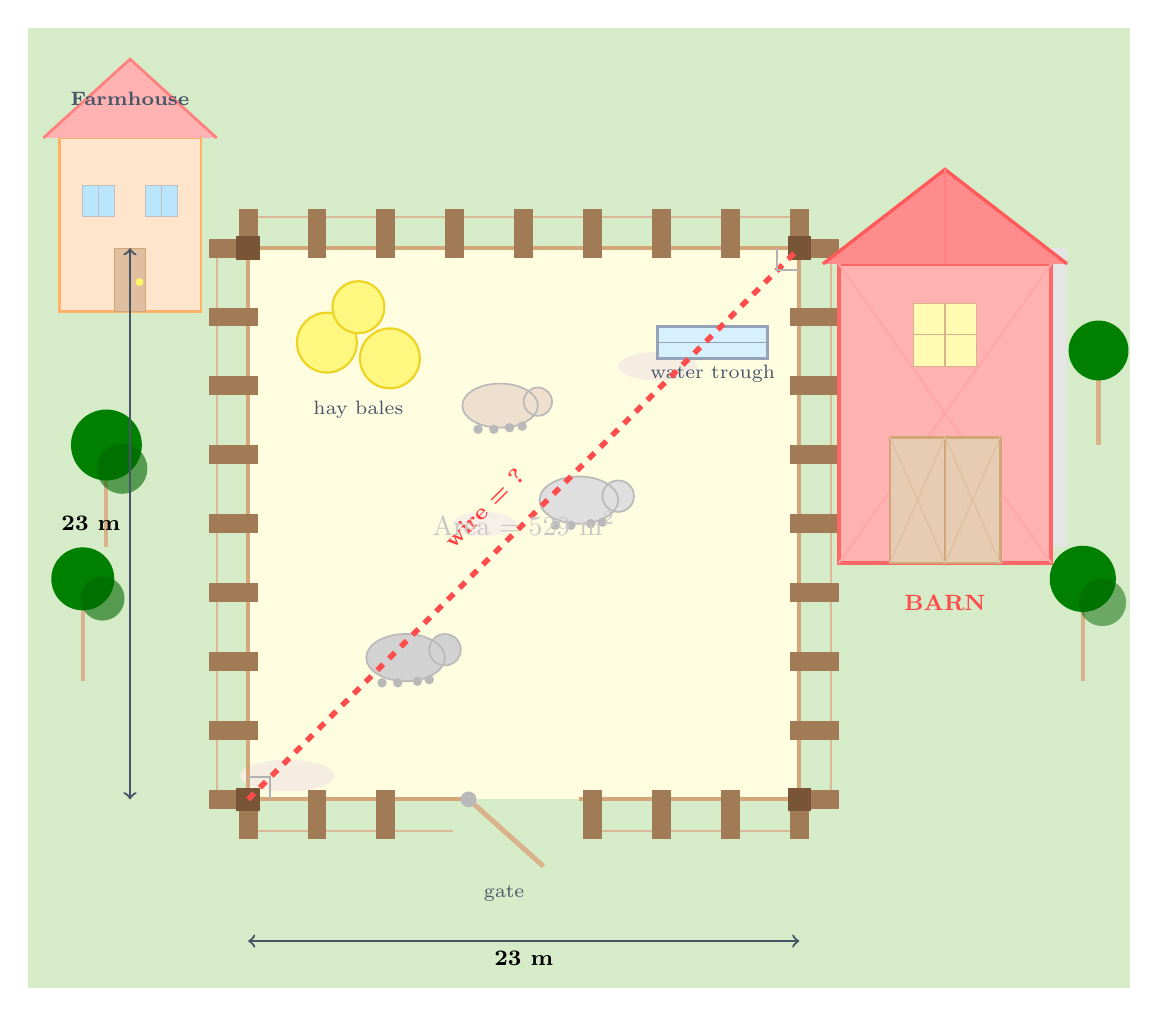
\begin{tikzpicture}[font=\small, scale=1.0]

  %% ---- BACKGROUND FIELD ----
  \fill[grass!60] (-2.8,-2.4) rectangle (11.2,9.8);

  %% ---- FARMHOUSE (upper left, outside pen) ----
  \fill[orange!20] (-2.4,6.2) rectangle (-0.6,8.4);
  \draw[orange!60, line width=1pt] (-2.4,6.2) rectangle (-0.6,8.4);
  % Roof
  \fill[red!30] (-2.6,8.4) -- (-1.5,9.4) -- (-0.4,8.4) -- cycle;
  \draw[red!50, line width=1pt] (-2.6,8.4) -- (-1.5,9.4) -- (-0.4,8.4);
  % Windows
  \fill[skyblue] (-2.1,7.4) rectangle (-1.7,7.8);
  \draw[gray!50] (-2.1,7.4) rectangle (-1.7,7.8);
  \draw[gray!50] (-1.9,7.4) -- (-1.9,7.8);
  \fill[skyblue] (-1.3,7.4) rectangle (-0.9,7.8);
  \draw[gray!50] (-1.3,7.4) rectangle (-0.9,7.8);
  \draw[gray!50] (-1.1,7.4) -- (-1.1,7.8);
  % Door
  \fill[brown!50] (-1.7,6.2) rectangle (-1.3,7.0);
  \draw[brown!70] (-1.7,6.2) rectangle (-1.3,7.0);
  \draw[brown!70] (-1.5,6.2) -- (-1.5,7.0);
  \fill[yellow!60] (-1.38,6.57) circle (0.05);
  \node[font=\scriptsize\bfseries, slate] at (-1.5,8.9) {Farmhouse};

  %% ---- TREES (left side) ----
  \draw[brown!60, line width=1.5pt] (-1.8,3.2) -- (-1.8,4.2);
  \fill[green!50!black] (-1.8,4.5) circle (0.45);
  \fill[green!40!black, opacity=0.6] (-1.6,4.2) circle (0.32);
  \draw[brown!60, line width=1.5pt] (-2.1,1.5) -- (-2.1,2.5);
  \fill[green!50!black] (-2.1,2.8) circle (0.4);
  \fill[green!40!black, opacity=0.6] (-1.85,2.55) circle (0.28);

  %% ---- SQUARE PEN ----

  % Pen ground fill (light dirt)
  \fill[yellow!12] (0,0) rectangle (7,7);

  % Mud patches (adds texture)
  \fill[brown!15] (0.5,0.3) ellipse (0.6 and 0.2);
  \fill[brown!15] (5.2,5.5) ellipse (0.5 and 0.18);
  \fill[brown!12] (3.0,3.5) ellipse (0.4 and 0.15);

  % Fence posts and rails — LEFT side
  \draw[brown!70, line width=1.5pt] (0,0) -- (0,7);
  \draw[brown!55, line width=0.7pt] (-0.4,0) -- (-0.4,7);
  \foreach \y in {0,0.875,1.75,2.625,3.5,4.375,5.25,6.125,7}
    \fill[earthbrown] (-0.5,\y-0.12) rectangle (0.12,\y+0.12);

  % Fence posts and rails — RIGHT side
  \draw[brown!70, line width=1.5pt] (7,0) -- (7,7);
  \draw[brown!55, line width=0.7pt] (7.4,0) -- (7.4,7);
  \foreach \y in {0,0.875,1.75,2.625,3.5,4.375,5.25,6.125,7}
    \fill[earthbrown] (6.88,\y-0.12) rectangle (7.5,\y+0.12);

  % Fence posts and rails — TOP
  \draw[brown!70, line width=1.5pt] (0,7) -- (7,7);
  \draw[brown!55, line width=0.7pt] (0,7.4) -- (7,7.4);
  \foreach \x in {0,0.875,1.75,2.625,3.5,4.375,5.25,6.125,7}
    \fill[earthbrown] (\x-0.12,6.88) rectangle (\x+0.12,7.5);

  % Fence — BOTTOM (with gate gap at x=2.8 to x=4.2)
  \draw[brown!70, line width=1.5pt] (0,0) -- (2.8,0);
  \draw[brown!70, line width=1.5pt] (4.2,0) -- (7,0);
  \draw[brown!55, line width=0.7pt] (0,-0.4) -- (2.6,-0.4);
  \draw[brown!55, line width=0.7pt] (4.4,-0.4) -- (7,-0.4);
  \foreach \x in {0,0.875,1.75}
    \fill[earthbrown] (\x-0.12,-0.5) rectangle (\x+0.12,0.12);
  \foreach \x in {4.375,5.25,6.125,7}
    \fill[earthbrown] (\x-0.12,-0.5) rectangle (\x+0.12,0.12);
  % Corner posts (chunkier)
  \fill[darkearth] (-0.15,-0.15) rectangle (0.15,0.15);
  \fill[darkearth] (6.85,-0.15) rectangle (7.15,0.15);
  \fill[darkearth] (-0.15,6.85) rectangle (0.15,7.15);
  \fill[darkearth] (6.85,6.85) rectangle (7.15,7.15);

  % GATE — opens inward, left-hinged at x=2.8
  \draw[brown!60, line width=1.8pt] (2.8,0) -- (3.75,-0.85);
  \draw[brown!60, line width=1pt]   (2.8,0) -- (3.35,-0.5);
  \draw[brown!60, line width=1pt]   (3.75,-0.85) -- (3.35,-0.5);
  \fill[gray!55] (2.8,0) circle (0.1);
  \node[font=\scriptsize, slate] at (3.25,-1.2) {gate};

  %% ---- WATER TROUGH ----
  \fill[skyblue!60] (5.2,5.6) rectangle (6.6,6.0);
  \draw[steelgray, line width=1pt] (5.2,5.6) rectangle (6.6,6.0);
  \draw[steelgray, line width=0.6pt] (5.2,5.8) -- (6.6,5.8);
  \node[font=\scriptsize, slate] at (5.9,5.4) {water trough};

  %% ---- HAY BALES (round, top-view) ----
  \fill[yellow!50] (1.0,5.8) circle (0.38);
  \draw[yellow!70!brown, line width=0.8pt] (1.0,5.8) circle (0.38);
  \fill[yellow!50] (1.8,5.6) circle (0.38);
  \draw[yellow!70!brown, line width=0.8pt] (1.8,5.6) circle (0.38);
  \fill[yellow!50] (1.4,6.25) circle (0.33);
  \draw[yellow!70!brown, line width=0.8pt] (1.4,6.25) circle (0.33);
  \node[font=\scriptsize, slate] at (1.4,4.95) {hay bales};

  %% ---- CATTLE (top-view silhouettes) ----
  % Cow 1
  \fill[gray!35] (2.0,1.8) ellipse (0.5 and 0.3);
  \fill[gray!35] (2.5,1.9) circle (0.2);
  \draw[gray!55, line width=0.6pt] (2.0,1.8) ellipse (0.5 and 0.3);
  \draw[gray!55, line width=0.6pt] (2.5,1.9) circle (0.2);
  \foreach \dx/\dy in {-0.3/-0.32, -0.1/-0.32, 0.15/-0.3, 0.3/-0.28}
    \fill[gray!55] (2.0+\dx, 1.8+\dy) circle (0.06);
  % Cow 2
  \fill[gray!25] (4.2,3.8) ellipse (0.5 and 0.3);
  \fill[gray!25] (4.7,3.85) circle (0.2);
  \draw[gray!55, line width=0.6pt] (4.2,3.8) ellipse (0.5 and 0.3);
  \draw[gray!55, line width=0.6pt] (4.7,3.85) circle (0.2);
  \foreach \dx/\dy in {-0.3/-0.32, -0.1/-0.32, 0.15/-0.3, 0.3/-0.28}
    \fill[gray!55] (4.2+\dx, 3.8+\dy) circle (0.06);
  % Cow 3
  \fill[brown!25] (3.2,5.0) ellipse (0.48 and 0.28);
  \fill[brown!25] (3.68,5.05) circle (0.18);
  \draw[gray!55, line width=0.6pt] (3.2,5.0) ellipse (0.48 and 0.28);
  \draw[gray!55, line width=0.6pt] (3.68,5.05) circle (0.18);
  \foreach \dx/\dy in {-0.28/-0.3, -0.08/-0.3, 0.12/-0.28, 0.28/-0.26}
    \fill[gray!55] (3.2+\dx, 5.0+\dy) circle (0.06);

  %% ---- BARN (upper right, outside pen) ----
  % Shadow
  \fill[black!10] (7.7,3.2) rectangle (10.4,7.0);
  % Walls
  \fill[red!30] (7.5,3.0) rectangle (10.2,6.8);
  \draw[red!60, line width=1.5pt] (7.5,3.0) rectangle (10.2,6.8);
  % Roof (isometric hint)
  \fill[red!45] (7.3,6.8) -- (8.85,8.0) -- (10.4,6.8) -- cycle;
  \draw[red!65, line width=1.2pt] (7.3,6.8) -- (8.85,8.0) -- (10.4,6.8);
  \draw[red!50, line width=0.7pt] (8.85,8.0) -- (8.85,6.8);  % ridge line
  % X-bracing on barn face
  \draw[red!35, line width=0.7pt] (7.5,3.0) -- (10.2,6.8);
  \draw[red!35, line width=0.7pt] (7.5,6.8) -- (10.2,3.0);
  % Barn door (double)
  \fill[brown!40] (8.15,3.0) rectangle (9.55,4.6);
  \draw[brown!70, line width=1pt] (8.15,3.0) rectangle (9.55,4.6);
  \draw[brown!70, line width=0.8pt] (8.85,3.0) -- (8.85,4.6);
  % X on doors
  \draw[brown!50, line width=0.5pt] (8.15,3.0) -- (8.85,4.6);
  \draw[brown!50, line width=0.5pt] (8.85,3.0) -- (8.15,4.6);
  \draw[brown!50, line width=0.5pt] (8.85,3.0) -- (9.55,4.6);
  \draw[brown!50, line width=0.5pt] (9.55,3.0) -- (8.85,4.6);
  % Hayloft window
  \fill[yellow!30] (8.45,5.5) rectangle (9.25,6.3);
  \draw[brown!60] (8.45,5.5) rectangle (9.25,6.3);
  \draw[brown!60] (8.85,5.5) -- (8.85,6.3);
  \draw[brown!60] (8.45,5.9) -- (9.25,5.9);
  \node[font=\footnotesize\bfseries, red!70] at (8.85,2.5) {BARN};

  %% ---- TREES (right side) ----
  \draw[brown!60, line width=1.5pt] (10.6,1.5) -- (10.6,2.5);
  \fill[green!50!black] (10.6,2.8) circle (0.42);
  \fill[green!40!black, opacity=0.5] (10.85,2.5) circle (0.3);
  \draw[brown!60, line width=1.5pt] (10.8,4.5) -- (10.8,5.4);
  \fill[green!50!black] (10.8,5.7) circle (0.38);

  %% ---- DIAGONAL SUPPORT WIRE ----
  \draw[red!70, line width=2pt, dashed] (0,0) -- (7,7);
  \node[red!75, font=\footnotesize\bfseries, rotate=45] at (3.0,3.7) {wire = ?};
  % Right-angle marks at corners
  \draw[gray!60, line width=0.7pt] (0.28,0) -- (0.28,0.28) -- (0,0.28);
  \draw[gray!60, line width=0.7pt] (6.72,7) -- (6.72,6.72) -- (7,6.72);

  %% ---- DIMENSION LABELS ----
  \draw[<->, slate, line width=0.8pt] (-1.5, 0) -- (-1.5, 7);
  \node[left, font=\footnotesize\bfseries] at (-1.5, 3.5) {23 m};
  \draw[<->, slate, line width=0.8pt] (0, -1.8) -- (7, -1.8);
  \node[below, font=\footnotesize\bfseries] at (3.5, -1.8) {23 m};
  % Area label (centre of pen)
  \node[gray!45, font=\normalsize] at (3.5,3.5) {Area $= 529\ \text{m}^2$};

\end{tikzpicture}
\end{center}

\begin{tcolorbox}[problem]
\textbf{Problem 1: The Ranch Corral}

\medskip
A rancher has built a square livestock corral with an area of \textbf{529~m$^2$}. She wants to run a
diagonal support wire from one corner of the corral to the opposite corner.

\medskip
\begin{enumerate}[label=(\alph*)]
  \item What is the side length of the corral? Show your work.

  \item What is the minimum length of wire needed for the diagonal? Round to the nearest tenth of a metre.
\end{enumerate}
\end{tcolorbox}

\begin{tcolorbox}[answerbox]
\textbf{(a)} \answerline\answerline
\textbf{(b)} \answerline\answerline\answerline
\end{tcolorbox}

\clearpage

% ============================================================
% PROBLEM 2 — RATIONAL NUMBERS — OIL WELL DRILLING
% ============================================================

\section*{Problem 2 \hfill \normalfont\small\color{slate}Rational Numbers}

\begin{center}
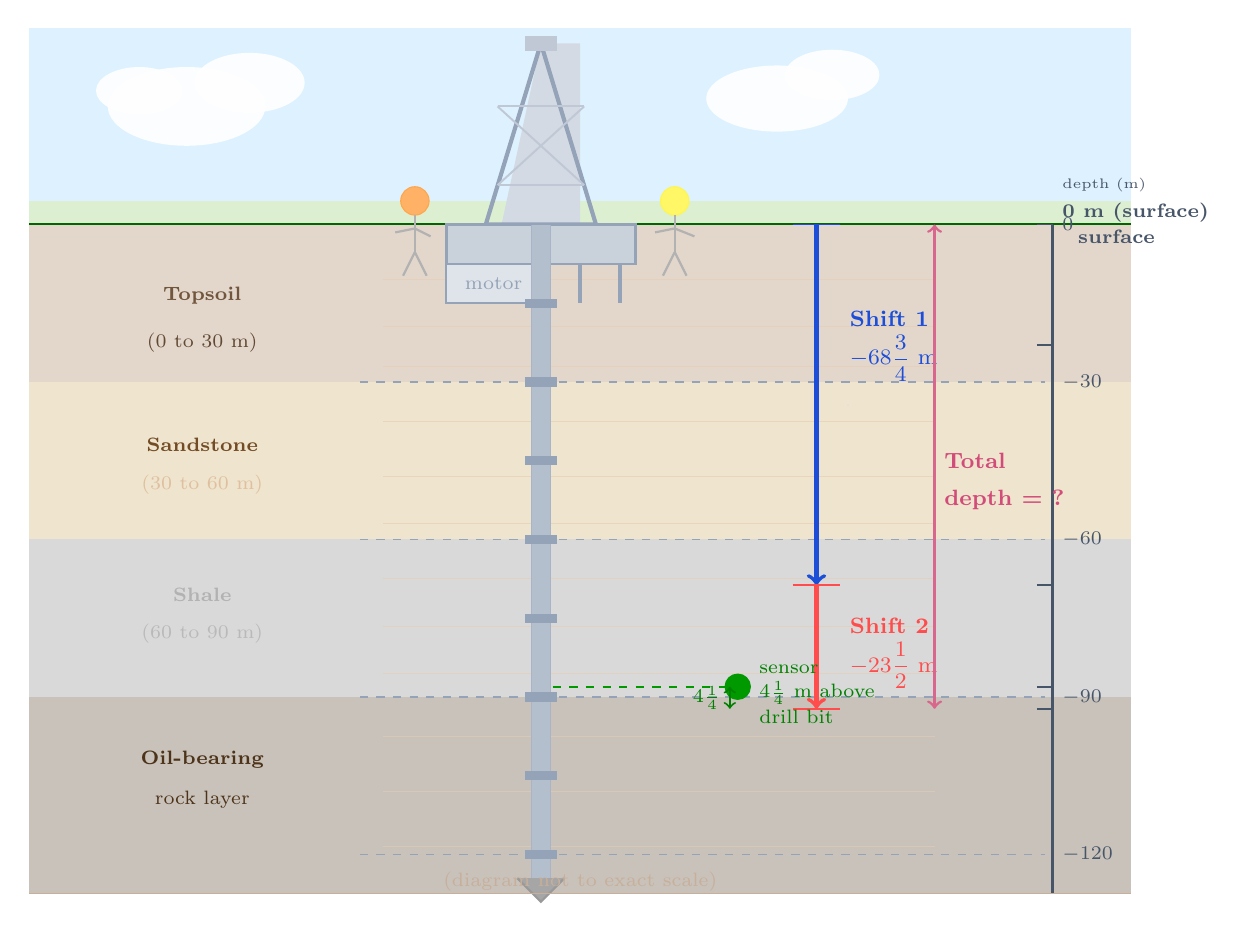
\begin{tikzpicture}[font=\small, scale=1.0]

  %% ---- SKY ----
  \fill[skyblue!50] (0,0) rectangle (14,2.5);
  % Clouds
  \fill[white, opacity=0.9] (2.0,1.5) ellipse (1.0 and 0.5);
  \fill[white, opacity=0.9] (2.8,1.8) ellipse (0.7 and 0.38);
  \fill[white, opacity=0.9] (1.4,1.7) ellipse (0.55 and 0.3);
  \fill[white, opacity=0.9] (9.5,1.6) ellipse (0.9 and 0.42);
  \fill[white, opacity=0.9] (10.2,1.9) ellipse (0.6 and 0.32);

  %% ---- SURFACE GROUND ----
  \fill[grass!70] (0,-0.5) rectangle (14,0);
  \fill[grass!50] (0,0) rectangle (14,0.3);
  % Ground line
  \draw[green!40!black, line width=1pt] (0,0) -- (14,0);

  %% ---- UNDERGROUND LAYERS ----
  % Layer 1: topsoil (0 to -2cm = 0 to -30m)
  \fill[earthbrown!30] (0,-2.0) rectangle (14,0);
  % Layer 2: sandstone (-30m to -60m)
  \fill[yellow!20!brown!30] (0,-4.0) rectangle (14,-2.0);
  \fill[gray!15, opacity=0.3] (0,-4.0) rectangle (14,-2.0);
  % Layer 3: shale (-60m to -90m)
  \fill[gray!30] (0,-6.0) rectangle (14,-4.0);
  % Layer 4: oil-bearing rock (-90m+)
  \fill[brown!40!black!30] (0,-8.5) rectangle (14,-6.0);
  % Rock texture (horizontal strata lines)
  \foreach \y in {-0.7,-1.3,-1.8,-2.5,-3.2,-3.8,-4.5,-5.1,-5.7,-6.5,-7.2,-7.9}
    \draw[white!60!brown, line width=0.4pt, opacity=0.6] (4.5,\y) -- (11.5,\y);

  %% ---- LAYER LABELS ----
  \node[font=\scriptsize\bfseries, earthbrown!70!black] at (2.2,-0.9) {Topsoil};
  \node[font=\scriptsize, earthbrown!60!black] at (2.2,-1.5) {(0 to 30 m)};
  \node[font=\scriptsize\bfseries, brown!60!black] at (2.2,-2.8) {Sandstone};
  \node[font=\scriptsize, brown!50] at (2.2,-3.3) {(30 to 60 m)};
  \node[font=\scriptsize\bfseries, gray!60] at (2.2,-4.7) {Shale};
  \node[font=\scriptsize, gray!55] at (2.2,-5.2) {(60 to 90 m)};
  \node[font=\scriptsize\bfseries, brown!40!black] at (2.2,-6.8) {Oil-bearing};
  \node[font=\scriptsize, brown!40!black] at (2.2,-7.3) {rock layer};

  %% ---- DEPTH SCALE (right side) ----
  \draw[slate, line width=1pt] (13.0,0) -- (13.0,-8.5);
  \foreach \y/\label in {0/0, -1.53/{$-23\frac{1}{2}$}, -4.58/{$-68\frac{3}{4}$}, -6.15/{$-92\frac{1}{4}$}, -5.87/{$-88$}}
    \draw[slate, line width=0.7pt] (12.8,\y) -- (13.0,\y);
  \node[right, font=\scriptsize\bfseries, slate] at (13.0,0.15) {0 m (surface)};
  \node[right, font=\scriptsize\bfseries, slate] at (13.2,-0.15) {surface};
  \foreach \y in {-2.0,-4.0,-6.0,-8.0}
    \draw[slatelight, line width=0.4pt, dashed] (4.2,\y) -- (12.9,\y);

  %% ---- DRILLING RIG ----
  % Derrick (triangular structure)
  \fill[steelgray!40] (6.0, 0) -- (7.0,0) -- (7.0, 2.3) -- (6.5, 2.3) -- cycle;
  % Derrick frame
  \draw[steelgray, line width=1.5pt] (5.8,0) -- (6.5,2.3) -- (7.2,0) -- cycle;
  % Cross-bracing on derrick
  \draw[steelgray!60, line width=0.7pt] (5.95,0.5) -- (7.05,1.5);
  \draw[steelgray!60, line width=0.7pt] (5.95,1.5) -- (7.05,0.5);
  \draw[steelgray!60, line width=0.7pt] (5.95,0.5) -- (7.05,0.5);
  \draw[steelgray!60, line width=0.7pt] (5.95,1.5) -- (7.05,1.5);
  % Rig platform
  \fill[steelgray!50] (5.3,-0.5) rectangle (7.7,0);
  \draw[steelgray, line width=1pt] (5.3,-0.5) rectangle (7.7,0);
  % Platform legs
  \draw[steelgray, line width=1.5pt] (5.5,-0.5) -- (5.5,-1.0);
  \draw[steelgray, line width=1.5pt] (6.0,-0.5) -- (6.0,-1.0);
  \draw[steelgray, line width=1.5pt] (7.0,-0.5) -- (7.0,-1.0);
  \draw[steelgray, line width=1.5pt] (7.5,-0.5) -- (7.5,-1.0);
  % Engine/motor house
  \fill[steelgray!30] (5.3,-1.0) rectangle (6.5,-0.5);
  \draw[steelgray, line width=0.8pt] (5.3,-1.0) rectangle (6.5,-0.5);
  \node[font=\scriptsize, steelgray] at (5.9,-0.75) {motor};
  % Crown block (top)
  \fill[steelgray!60] (6.3,2.2) rectangle (6.7,2.4);

  %% ---- DRILL PIPE ----
  \fill[steelgray!70] (6.38,0) rectangle (6.62,-8.3);
  \draw[steelgray!80, line width=0.5pt] (6.38,0) -- (6.38,-8.3);
  \draw[steelgray!80, line width=0.5pt] (6.62,0) -- (6.62,-8.3);
  % Pipe couplings
  \foreach \y in {-1,-2,-3,-4,-5,-6,-7,-8}
    \fill[steelgray] (6.3,\y-0.06) rectangle (6.7,\y+0.06);
  % Drill bit at bottom
  \fill[gray!70] (6.2,-8.3) -- (6.5,-8.6) -- (6.8,-8.3) -- cycle;
  \draw[gray!80, line width=0.8pt] (6.2,-8.3) -- (6.5,-8.6) -- (6.8,-8.3);

  %% ---- WORKERS ----
  % Worker 1 (left of rig)
  \fill[orange!60] (4.9,0.3) circle (0.18);  % hardhat
  \draw[orange!70] (4.9,0.3) circle (0.18);
  \draw[gray!60, line width=0.8pt] (4.9,0.12) -- (4.9,-0.35); % body
  \draw[gray!60, line width=0.8pt] (4.65,-0.1) -- (4.9,-0.05) -- (5.1,-0.15); % arms
  \draw[gray!60, line width=0.8pt] (4.9,-0.35) -- (4.75,-0.65);
  \draw[gray!60, line width=0.8pt] (4.9,-0.35) -- (5.05,-0.65);
  % Worker 2 (right of rig)
  \fill[yellow!60] (8.2,0.3) circle (0.18);
  \draw[yellow!70] (8.2,0.3) circle (0.18);
  \draw[gray!60, line width=0.8pt] (8.2,0.12) -- (8.2,-0.35);
  \draw[gray!60, line width=0.8pt] (7.95,-0.1) -- (8.2,-0.05) -- (8.45,-0.15);
  \draw[gray!60, line width=0.8pt] (8.2,-0.35) -- (8.05,-0.65);
  \draw[gray!60, line width=0.8pt] (8.2,-0.35) -- (8.35,-0.65);

  %% ---- MEASUREMENT ANNOTATIONS ----

  % First shift: 0 to -68¾m (scale: 1cm = ~15m, so -68.75m ≈ -4.58cm)
  \draw[accent, line width=1.5pt, ->] (10.0, 0) -- (10.0,-4.58);
  \draw[accent, line width=0.7pt] (9.7,0) -- (10.3,0);
  \draw[accent, line width=0.7pt] (9.7,-4.58) -- (10.3,-4.58);
  \fill[accent!20] (10.4,-2.29) circle (0.01);
  \node[right, font=\footnotesize\bfseries\color{accent}] at (10.3,-1.2) {Shift 1};
  \node[right, font=\footnotesize\color{accent}] at (10.3,-1.7) {$-68\dfrac{3}{4}$ m};

  % Second shift: -68¾m to -92¼m (additional -23½m, so from -4.58 to -6.15cm)
  \draw[red!70, line width=1.5pt, ->] (10.0,-4.58) -- (10.0,-6.15);
  \draw[red!70, line width=0.7pt] (9.7,-4.58) -- (10.3,-4.58);
  \draw[red!70, line width=0.7pt] (9.7,-6.15) -- (10.3,-6.15);
  \node[right, font=\footnotesize\bfseries\color{red!70}] at (10.3,-5.1) {Shift 2};
  \node[right, font=\footnotesize\color{red!70}] at (10.3,-5.6) {$-23\dfrac{1}{2}$ m};

  % Sensor position: 4¼m above drill bit = -88m = -5.87cm from surface
  \fill[green!60!black] (9.0,-5.87) circle (0.15);
  \draw[green!60!black, line width=1pt] (9.0,-5.87) circle (0.15);
  \draw[green!60!black, line width=0.8pt, dashed] (6.65,-5.87) -- (9.0,-5.87);
  \node[right, font=\scriptsize\color{green!50!black}] at (9.15,-5.65) {sensor};
  \node[right, font=\scriptsize\color{green!50!black}] at (9.15,-5.95) {$4\tfrac{1}{4}$ m above};
  \node[right, font=\scriptsize\color{green!50!black}] at (9.15,-6.25) {drill bit};
  % Arrow from sensor to drill bit
  \draw[green!50!black, <->, line width=0.7pt] (8.9,-5.87) -- (8.9,-6.15);
  \node[left, font=\scriptsize\color{green!50!black}] at (8.9,-6.01) {$4\tfrac{1}{4}$};

  % Total depth label
  \draw[purple!60, line width=1pt, <->] (11.5,0) -- (11.5,-6.15);
  \node[right, font=\footnotesize\bfseries\color{purple!70}] at (11.5,-3.0) {Total};
  \node[right, font=\footnotesize\bfseries\color{purple!70}] at (11.5,-3.5) {depth = ?};

  %% ---- DEPTH NUMBERS (right scale) ----
  \node[right, font=\scriptsize, slate] at (13.0, 0)    {0};
  \node[right, font=\scriptsize, slate] at (13.0,-2.0)  {$-30$};
  \node[right, font=\scriptsize, slate] at (13.0,-4.0)  {$-60$};
  \node[right, font=\scriptsize, slate] at (13.0,-6.0)  {$-90$};
  \node[right, font=\scriptsize, slate] at (13.0,-8.0)  {$-120$};
  \node[right, font=\tiny, slate] at (13.0,0.5) {depth (m)};

  %% ---- BOTTOM BORDER ----
  \draw[earthbrown!60] (0,-8.5) -- (14,-8.5);
  \node[font=\scriptsize, earthbrown!60] at (7,-8.35) {(diagram not to exact scale)};

\end{tikzpicture}
\end{center}

\begin{tcolorbox}[problem]
\textbf{Problem 2: Going Deep}

\medskip
An oil drilling crew starts at the surface (depth~$= 0$~m). During the first shift, they drill
down $68\dfrac{3}{4}$~m. During the second shift, they drill an additional $23\dfrac{1}{2}$~m deeper.
A pressure sensor is attached to the drill pipe $4\dfrac{1}{4}$~m \emph{above} the drill bit.

\medskip
\begin{enumerate}[label=(\alph*)]
  \item What is the total depth of the drill bit after both shifts? Express your answer as a mixed number.

  \item What is the depth of the pressure sensor? Express your answer as a mixed number.
\end{enumerate}
\end{tcolorbox}

\begin{tcolorbox}[answerbox]
\textbf{(a)} \answerline\answerline
\textbf{(b)} \answerline\answerline
\end{tcolorbox}

\clearpage

% ============================================================
% PROBLEM 3 — POWERS & EXPONENTS — BACTERIA CULTURE
% ============================================================

\section*{Problem 3 \hfill \normalfont\small\color{slate}Powers \& Exponents}

\begin{center}
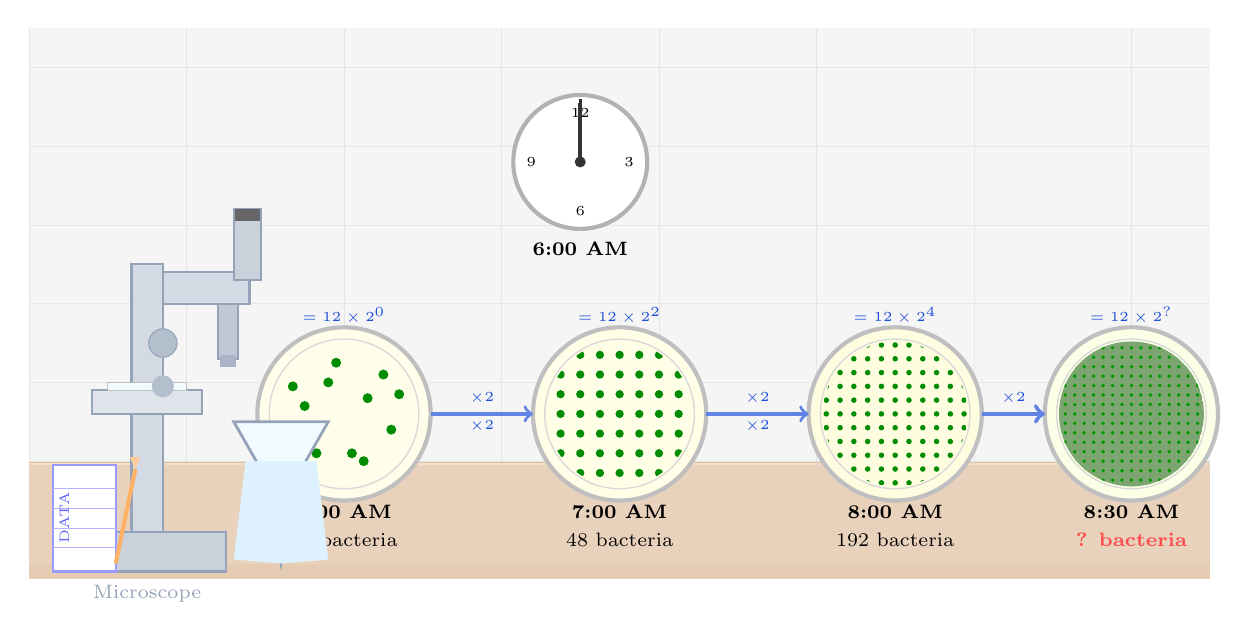
\begin{tikzpicture}[font=\small, scale=1.0]

  %% ---- LAB BENCH SURFACE ----
  \fill[brown!25] (0,-1.5) rectangle (15,0);
  \fill[brown!35] (0,-1.5) rectangle (15,-0.05);
  \draw[brown!50, line width=1pt] (0,0) -- (15,0);
  % Bench front edge (lip)
  \fill[brown!40] (0,-1.5) rectangle (15,-1.3);

  %% ---- WALL BEHIND BENCH ----
  \fill[gray!8] (0,0) rectangle (15,5.5);
  % Wall tiles (faint grid)
  \foreach \x in {0,2,4,6,8,10,12,14}
    \draw[gray!20, line width=0.3pt] (\x,0) -- (\x,5.5);
  \foreach \y in {0,1,2,3,4,5}
    \draw[gray!20, line width=0.3pt] (0,\y) -- (15,\y);

  %% ---- CLOCK ON WALL (top centre) ----
  \fill[white] (7.0,3.8) circle (0.85);
  \draw[gray!60, line width=1.5pt] (7.0,3.8) circle (0.85);
  % Clock numbers
  \foreach \h/\angle in {12/90, 3/0, 6/270, 9/180}
    \node[font=\tiny] at ({7.0 + 0.62*cos(\angle)}, {3.8 + 0.62*sin(\angle)}) {\h};
  % Clock hands — showing 6:00 AM
  \draw[black!80, line width=1.5pt] (7.0,3.8) -- (7.0,4.55);  % hour hand (up = 12)
  \draw[black!80, line width=1.0pt] (7.0,3.8) -- (7.0,4.6);   % minute hand (12)
  \fill[black!80] (7.0,3.8) circle (0.07);
  \node[below, font=\scriptsize\bfseries] at (7.0,2.9) {6:00 AM};

  %% ---- MICROSCOPE (left side of bench) ----
  % Base
  \fill[steelgray!50] (0.5,-1.4) rectangle (2.5,-0.9);
  \draw[steelgray, line width=1pt] (0.5,-1.4) rectangle (2.5,-0.9);
  % Arm (vertical + horizontal)
  \fill[steelgray!40] (1.3,-0.9) rectangle (1.7,2.5);  % vertical arm
  \draw[steelgray, line width=0.8pt] (1.3,-0.9) rectangle (1.7,2.5);
  \fill[steelgray!40] (1.7,2.0) rectangle (2.8,2.4);   % horizontal arm
  \draw[steelgray, line width=0.8pt] (1.7,2.0) rectangle (2.8,2.4);
  % Stage (horizontal platform for slide)
  \fill[steelgray!30] (0.8,0.6) rectangle (2.2,0.9);
  \draw[steelgray, line width=0.8pt] (0.8,0.6) rectangle (2.2,0.9);
  % Slide on stage
  \fill[skyblue!20] (1.0,0.9) rectangle (2.0,1.0);
  \draw[gray!50] (1.0,0.9) rectangle (2.0,1.0);
  % Objective lens (hanging down from arm)
  \fill[steelgray!60] (2.4,1.3) rectangle (2.65,2.0);
  \draw[steelgray, line width=0.7pt] (2.4,1.3) rectangle (2.65,2.0);
  \fill[steelgray!80] (2.42,1.2) rectangle (2.63,1.35);
  % Eyepiece (top)
  \fill[steelgray!50] (2.6,2.3) rectangle (2.95,3.2);
  \draw[steelgray, line width=0.8pt] (2.6,2.3) rectangle (2.95,3.2);
  \fill[black!60] (2.62,3.05) rectangle (2.93,3.2);
  % Focus knobs
  \fill[steelgray!70] (1.7,1.5) circle (0.18);
  \draw[steelgray] (1.7,1.5) circle (0.18);
  \fill[steelgray!70] (1.7,0.95) circle (0.14);
  \node[below, font=\scriptsize, steelgray] at (1.5,-1.45) {Microscope};

  %% ---- PETRI DISH HELPER STYLE ----
  % We draw 4 dishes showing bacterial growth at 4 time points

  % --- Dish 1: 6:00 AM — 12 bacteria ---
  \coordinate (D1) at (4.0,0.6);
  \fill[yellow!8] (D1) circle (1.1);
  \draw[gray!50, line width=1.5pt] (D1) circle (1.1);
  \draw[gray!30, line width=0.5pt] (D1) circle (0.95);  % inner wall
  % 12 bacteria (manually placed, large)
  \begin{scope}
    \clip (D1) circle (0.92);
    \foreach \bx/\by in {
      0.3/0.2, -0.2/0.4, 0.1/-0.5, -0.5/0.1, 0.6/-0.2,
      -0.1/0.65, 0.5/0.5, -0.6/-0.2, 0.25/-0.6, -0.35/-0.5,
      -0.65/0.35, 0.7/0.25}
      \fill[green!55!black] ({4.0+\bx},{0.6+\by}) circle (1.8pt);
  \end{scope}
  % Label
  \node[below, font=\scriptsize\bfseries] at (D1) {};
  \node[font=\scriptsize\bfseries] at (4.0,-0.65) {6:00 AM};
  \node[font=\scriptsize] at (4.0,-1.0) {12 bacteria};
  \node[font=\tiny, accent] at (4.0,1.85) {$= 12 \times 2^0$};

  % --- Dish 2: 7:00 AM — 48 bacteria (2 doublings = ×4) ---
  \coordinate (D2) at (7.5,0.6);
  \fill[yellow!10] (D2) circle (1.1);
  \draw[gray!50, line width=1.5pt] (D2) circle (1.1);
  \draw[gray!30, line width=0.5pt] (D2) circle (0.95);
  \begin{scope}
    \clip (D2) circle (0.92);
    \foreach \i in {-3,-2,-1,0,1,2,3}
      \foreach \j in {-3,-2,-1,0,1,2,3}
        \fill[green!55!black] ({7.5+\i*0.25},{0.6+\j*0.25}) circle (1.5pt);
  \end{scope}
  \node[font=\scriptsize\bfseries] at (7.5,-0.65) {7:00 AM};
  \node[font=\scriptsize] at (7.5,-1.0) {48 bacteria};
  \node[font=\tiny, accent] at (7.5,1.85) {$= 12 \times 2^2$};

  % --- Dish 3: 8:00 AM — 192 bacteria (4 doublings = ×16) ---
  \coordinate (D3) at (11.0,0.6);
  \fill[yellow!12] (D3) circle (1.1);
  \draw[gray!50, line width=1.5pt] (D3) circle (1.1);
  \draw[gray!30, line width=0.5pt] (D3) circle (0.95);
  \begin{scope}
    \clip (D3) circle (0.92);
    \foreach \i in {-5,-4,...,5}
      \foreach \j in {-5,-4,...,5}
        \fill[green!55!black] ({11.0+\i*0.175},{0.6+\j*0.175}) circle (1.0pt);
  \end{scope}
  \node[font=\scriptsize\bfseries] at (11.0,-0.65) {8:00 AM};
  \node[font=\scriptsize] at (11.0,-1.0) {192 bacteria};
  \node[font=\tiny, accent] at (11.0,1.85) {$= 12 \times 2^4$};

  % --- Dish 4: 8:30 AM — 384 bacteria (5 doublings = ×32) ---
  \coordinate (D4) at (14.0,0.6);
  \fill[green!15!yellow!10] (D4) circle (1.1);
  \draw[gray!50, line width=1.5pt] (D4) circle (1.1);
  \draw[gray!30, line width=0.5pt] (D4) circle (0.95);
  \begin{scope}
    \clip (D4) circle (0.92);
    % Very dense fill
    \fill[green!30!black, opacity=0.5] (D4) circle (0.92);
    \foreach \i in {-7,-6,...,7}
      \foreach \j in {-7,-6,...,7}
        \fill[green!60!black] ({14.0+\i*0.12},{0.6+\j*0.12}) circle (0.7pt);
  \end{scope}
  \node[font=\scriptsize\bfseries] at (14.0,-0.65) {8:30 AM};
  \node[font=\scriptsize\bfseries, red!70] at (14.0,-1.0) {? bacteria};
  \node[font=\tiny, accent] at (14.0,1.85) {$= 12 \times 2^?$};

  %% ---- ARROWS BETWEEN DISHES (doubling) ----
  \foreach \xa/\xb in {5.1/6.4, 8.6/9.9, 12.1/12.9}
    \draw[->, accent!70, line width=1.2pt] (\xa,0.6) -- (\xb,0.6);
  \node[above, font=\tiny, accent] at (5.75,0.6) {$\times 2$};
  \node[above, font=\tiny, accent] at (5.75,0.25) {$\times 2$};
  \node[above, font=\tiny, accent] at (9.25,0.6) {$\times 2$};
  \node[above, font=\tiny, accent] at (9.25,0.25) {$\times 2$};
  \draw[->, accent!70, line width=1.5pt] (12.1,0.6) -- (12.9,0.6);
  \node[above, font=\tiny, accent] at (12.5,0.6) {$\times 2$};

  %% ---- BEAKER / FLASK on bench (right area) ----
  % Erlenmeyer flask
  \fill[skyblue!20] (3.2,-1.3) -- (3.0,-0.2) -- (2.6,0.5) -- (3.8,0.5) -- (3.4,-0.2) -- (3.2,-1.3);
  \draw[steelgray, line width=1pt] (3.2,-1.3) -- (3.0,-0.2) -- (2.6,0.5) -- (3.8,0.5) -- (3.4,-0.2) -- (3.2,-1.3) -- cycle;
  \draw[steelgray, line width=0.6pt] (2.75,-0.05) -- (3.65,-0.05);
  \fill[skyblue!50] (2.6,-1.25) -- (3.2,-1.3) -- (3.8,-1.25) -- (3.65,-0.0) -- (2.75,-0.0) -- cycle;

  %% ---- NOTEBOOK (bench) ----
  \fill[white] (0.3,-1.4) rectangle (1.1,-0.05);
  \draw[blue!40, line width=0.8pt] (0.3,-1.4) rectangle (1.1,-0.05);
  \draw[blue!30, line width=0.4pt] (0.3,-0.35) -- (1.1,-0.35);
  \draw[blue!30, line width=0.4pt] (0.3,-0.6) -- (1.1,-0.6);
  \draw[blue!30, line width=0.4pt] (0.3,-0.85) -- (1.1,-0.85);
  \draw[blue!30, line width=0.4pt] (0.3,-1.1) -- (1.1,-1.1);
  \node[font=\tiny, blue!60, rotate=90] at (0.45,-0.72) {DATA};
  % Pen/pencil on notebook
  \draw[orange!60, line width=1.5pt] (1.1,-1.3) -- (1.35,-0.1);
  \fill[orange!40] (1.35,-0.1) -- (1.28,0.05) -- (1.41,0.05) -- cycle;

\end{tikzpicture}
\end{center}

\begin{tcolorbox}[problem]
\textbf{Problem 3: Bacterial Explosion}

\medskip
A biology student places \textbf{12 bacteria} in a culture dish at \textbf{6:00 AM}. The bacteria
double every \textbf{30 minutes}.

\medskip
\begin{enumerate}[label=(\alph*)]
  \item How many doubling periods occur between 6:00 AM and 8:30 AM?

  \item Write an expression using a \textbf{power} (exponent) for the number of bacteria at 8:30 AM.

  \item Evaluate your expression. How many bacteria are in the dish at 8:30 AM?
\end{enumerate}
\end{tcolorbox}

\begin{tcolorbox}[answerbox]
\textbf{(a)} \answerline
\textbf{(b)} \answerline
\textbf{(c)} \answerline\answerline
\end{tcolorbox}

\clearpage

% ============================================================
% PROBLEM 4 — RATIONAL NUMBERS (×÷ mixed numbers) — WHEAT FARM
% ============================================================

\section*{Problem 4 \hfill \normalfont\small\color{slate}Rational Numbers}

\begin{center}
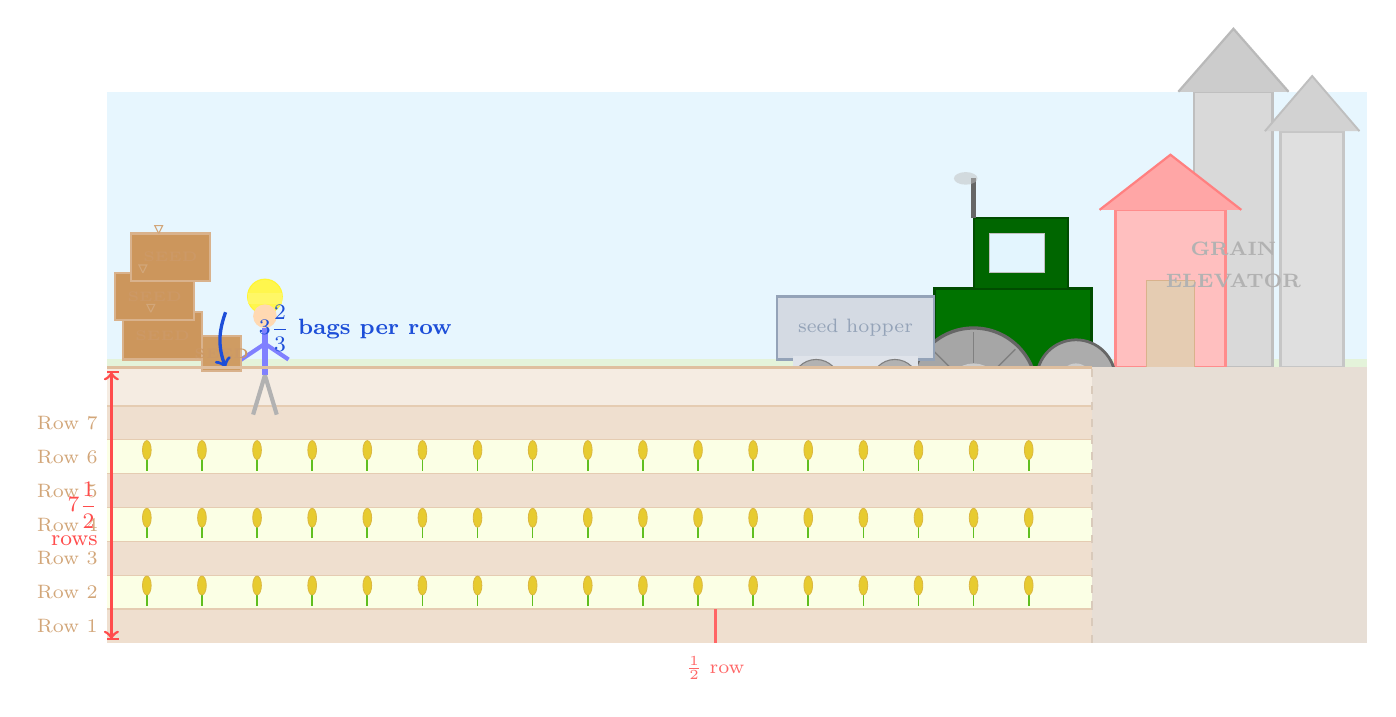
\begin{tikzpicture}[font=\small, scale=1.0]

  %% ---- SKY AND GROUND ----
  \fill[skyblue!35] (0,3.5) rectangle (16,7.0);
  \fill[grass!40] (0,3.2) rectangle (16,3.6);

  %% ---- GRAIN ELEVATOR / BARN (far right) ----
  % Main bin (tall cylinder rendered as rectangle)
  \fill[gray!30] (13.8,3.5) rectangle (14.8,7.0);
  \draw[gray!50, line width=1pt] (13.8,3.5) rectangle (14.8,7.0);
  % Bin top (roof cone = triangle)
  \fill[gray!40] (13.6,7.0) -- (14.3,7.8) -- (15.0,7.0) -- cycle;
  \draw[gray!55, line width=0.8pt] (13.6,7.0) -- (14.3,7.8) -- (15.0,7.0);
  % Second bin
  \fill[gray!25] (14.9,3.5) rectangle (15.7,6.5);
  \draw[gray!45, line width=1pt] (14.9,3.5) rectangle (15.7,6.5);
  \fill[gray!35] (14.7,6.5) -- (15.3,7.2) -- (15.9,6.5) -- cycle;
  \draw[gray!50, line width=0.7pt] (14.7,6.5) -- (15.3,7.2) -- (15.9,6.5);
  % Loading shed
  \fill[red!25] (12.8,3.5) rectangle (14.2,5.5);
  \draw[red!45, line width=1pt] (12.8,3.5) rectangle (14.2,5.5);
  \fill[red!35] (12.6,5.5) -- (13.5,6.2) -- (14.4,5.5) -- cycle;
  \draw[red!50, line width=0.8pt] (12.6,5.5) -- (13.5,6.2) -- (14.4,5.5);
  % Shed door
  \fill[brown!40] (13.2,3.5) rectangle (13.8,4.6);
  \draw[brown!60] (13.2,3.5) rectangle (13.8,4.6);
  \node[font=\scriptsize\bfseries, gray!60] at (14.3,5.0) {GRAIN};
  \node[font=\scriptsize\bfseries, gray!60] at (14.3,4.6) {ELEVATOR};

  %% ---- TRACTOR (middle right) ----
  % Body
  \fill[green!45!black] (10.5,3.5) rectangle (12.5,4.5);
  \draw[green!30!black, line width=1pt] (10.5,3.5) rectangle (12.5,4.5);
  % Cab
  \fill[green!40!black] (11.0,4.5) rectangle (12.2,5.4);
  \draw[green!30!black, line width=0.8pt] (11.0,4.5) rectangle (12.2,5.4);
  % Cab windows
  \fill[skyblue!40] (11.2,4.7) rectangle (11.9,5.2);
  \draw[gray!50] (11.2,4.7) rectangle (11.9,5.2);
  % Rear wheel (large)
  \fill[gray!70] (11.0,3.2) circle (0.8);
  \draw[black!60, line width=1.2pt] (11.0,3.2) circle (0.8);
  \fill[gray!40] (11.0,3.2) circle (0.35);
  % Spokes
  \foreach \a in {0,45,90,135,180,225,270,315}
    \draw[black!50, line width=0.5pt] ({11.0+0.35*cos(\a)},{3.2+0.35*sin(\a)}) --
                                      ({11.0+0.75*cos(\a)},{3.2+0.75*sin(\a)});
  % Front wheel (smaller)
  \fill[gray!65] (12.3,3.35) circle (0.5);
  \draw[black!60, line width=1pt] (12.3,3.35) circle (0.5);
  \fill[gray!40] (12.3,3.35) circle (0.2);
  % Exhaust pipe
  \draw[black!60, line width=2pt] (11.0,5.4) -- (11.0,5.9);
  \fill[gray!50, opacity=0.5] (10.9,5.9) ellipse (0.15 and 0.08);
  % Seed hopper (trailer behind tractor)
  \fill[steelgray!40] (8.5,3.6) rectangle (10.5,4.4);
  \draw[steelgray, line width=0.8pt] (8.5,3.6) rectangle (10.5,4.4);
  \fill[steelgray!30] (8.7,3.4) rectangle (10.3,3.65);
  % Hopper wheels
  \fill[gray!60] (9.0,3.3) circle (0.3);
  \draw[black!50] (9.0,3.3) circle (0.3);
  \fill[gray!60] (10.0,3.3) circle (0.3);
  \draw[black!50] (10.0,3.3) circle (0.3);
  \node[font=\scriptsize, steelgray] at (9.5,4.0) {seed hopper};

  %% ---- FIELD (lower portion) ----
  % Field background
  \fill[brown!15] (0,0) rectangle (16,3.5);

  % Row colors (alternating planted/unplanted)
  \foreach \row/\col in {
    0/brown!25, 1/green!15!yellow!10, 2/brown!25, 3/green!15!yellow!10,
    4/brown!25, 5/green!15!yellow!10, 6/brown!25}
    \fill[\col] (0,{0.43*\row}) rectangle (16,{0.43*(\row+1)});

  % Row dividers
  \foreach \y in {0.43, 0.86, 1.29, 1.72, 2.15, 2.58, 3.01}
    \draw[brown!40, line width=0.5pt] (0,\y) -- (16,\y);

  % Wheat plants in rows 1, 3, 5 (the planted rows)
  \foreach \row in {1, 3, 5} {
    \foreach \x in {0.5, 1.2, 1.9, 2.6, 3.3, 4.0, 4.7, 5.4, 6.1, 6.8,
                    7.5, 8.2, 8.9, 9.6, 10.3, 11.0, 11.7} {
      % Wheat stalk
      \draw[green!50!brown, line width=0.6pt]
        (\x, {0.43*\row + 0.04}) -- (\x, {0.43*\row + 0.3});
      % Wheat head
      \fill[yellow!60!brown] (\x, {0.43*\row + 0.3}) ellipse (0.055 and 0.12);
      \draw[yellow!40!brown, line width=0.3pt] (\x, {0.43*\row + 0.3}) ellipse (0.055 and 0.12);
    }
  }

  % Row number labels (left side)
  \foreach \row/\label in {0/1, 1/2, 2/3, 3/4, 4/5, 5/6, 6/7} {
    \node[left, font=\scriptsize, brown!70] at (0.0, {0.43*\row + 0.215}) {Row \label};
  }
  % Last row partial indicator
  \draw[red!60, line width=1pt] (7.72,0) -- (7.72,0.43);
  \node[below, font=\scriptsize\color{red!60}] at (7.72,-0.05) {$\frac{1}{2}$ row};

  %% ---- SEED BAGS PILE (left side) ----
  % Stack of bags
  \fill[burlywood!40!brown] (0.2,3.6) rectangle (1.2,4.2);
  \draw[brown!60, line width=0.8pt] (0.2,3.6) rectangle (1.2,4.2);
  \fill[burlywood!40!brown] (0.1,4.1) rectangle (1.1,4.7);
  \draw[brown!60, line width=0.8pt] (0.1,4.1) rectangle (1.1,4.7);
  \fill[burlywood!40!brown] (0.3,4.6) rectangle (1.3,5.2);
  \draw[brown!60, line width=0.8pt] (0.3,4.6) rectangle (1.3,5.2);
  % Bag labels
  \node[font=\tiny\bfseries, brown!80] at (0.7,3.9) {SEED};
  \node[font=\tiny\bfseries, brown!80] at (0.6,4.4) {SEED};
  \node[font=\tiny\bfseries, brown!80] at (0.8,4.9) {SEED};
  % Bag tie tops
  \draw[brown!70] (0.55,4.2) -- (0.5,4.3) -- (0.6,4.3) -- (0.55,4.2);
  \draw[brown!70] (0.45,4.7) -- (0.4,4.8) -- (0.5,4.8) -- (0.45,4.7);
  \draw[brown!70] (0.65,5.2) -- (0.6,5.3) -- (0.7,5.3) -- (0.65,5.2);

  %% ---- WORKER with bag ----
  % Worker standing at start of field (left side)
  % Hardhat
  \fill[yellow!70] (2.0,4.4) circle (0.22);
  \draw[yellow!80] (2.0,4.4) circle (0.22);
  \fill[yellow!60] (1.78,4.3) rectangle (2.22,4.44);
  % Head
  \fill[orange!30] (2.0,4.15) circle (0.15);
  % Body
  \draw[blue!50, line width=2pt] (2.0,4.0) -- (2.0,3.4);
  % Arms
  \draw[blue!50, line width=1.5pt] (2.0,3.8) -- (1.7,3.6) -- (1.5,3.65); % left arm
  \draw[blue!50, line width=1.5pt] (2.0,3.8) -- (2.3,3.6); % right arm
  % Seed bag in hand
  \fill[burlywood!50!brown] (1.2,3.45) rectangle (1.7,3.9);
  \draw[brown!60, line width=0.7pt] (1.2,3.45) rectangle (1.7,3.9);
  \node[font=\tiny\bfseries, brown!80] at (1.45,3.67) {SEED};
  % Legs
  \draw[gray!60, line width=1.5pt] (2.0,3.4) -- (1.85,2.9);
  \draw[gray!60, line width=1.5pt] (2.0,3.4) -- (2.15,2.9);

  %% ---- ANNOTATION: BAGS PER ROW ----
  % Arrow from bags to row with label
  \draw[accent, line width=1.2pt, ->] (1.5,4.2) to[bend right=20] (1.5,3.5);
  \node[right, font=\footnotesize\bfseries\color{accent}] at (1.8,4.0) {$3\dfrac{2}{3}$ bags per row};

  %% ---- ANNOTATION: NUMBER OF ROWS ----
  \draw[<->, red!70, line width=1pt] (0.05,0.05) -- (0.05,3.44);
  \draw[red!70, line width=0.5pt] (0.0,3.44) -- (0.15,3.44);
  \draw[red!70, line width=0.5pt] (0.0,0.05) -- (0.15,0.05);
  \node[left, font=\footnotesize\bfseries\color{red!70}] at (0.0, 1.75) {$7\dfrac{1}{2}$};
  \node[left, font=\footnotesize\color{red!70}] at (0.0, 1.3) {rows};

  %% ---- HORIZON / FIELD EDGE LINE ----
  \draw[brown!50, line width=1pt] (0,3.5) -- (12.5,3.5);

  %% ---- DIRT PATH to elevator ----
  \fill[earthbrown!25] (12.5,3.5) -- (12.5,0) -- (16,0) -- (16,3.5) -- cycle;
  \draw[earthbrown!40, line width=0.8pt, dashed] (12.5,0) -- (12.5,3.5);

\end{tikzpicture}
\end{center}

\begin{tcolorbox}[problem]
\textbf{Problem 4: Seeding the Field}

\medskip
A farmer is seeding a wheat field. Each row of the field requires exactly $3\dfrac{2}{3}$ bags of
seed. The field has $7\dfrac{1}{2}$ rows to plant.

\medskip
\begin{enumerate}[label=(\alph*)]
  \item Write a multiplication expression for the total number of bags of seed needed.
  Convert both mixed numbers to improper fractions and solve. Express your answer as a mixed number.

  \item Bags of seed cost \$28.50 each. If the farmer can only purchase whole bags, what is the total
  cost to buy enough seed to plant the entire field?
\end{enumerate}
\end{tcolorbox}

\begin{tcolorbox}[answerbox]
\textbf{(a)} \answerline\answerline\answerline
\textbf{(b)} \answerline\answerline
\end{tcolorbox}

\end{document}
